\section*{Results and Discussion}
\subsection*{Statistics}
The model we used in this experiment was that the distribution of the measurements of the lifetime of the muon, is distributed as an exponentially distributed random variable. This means that our model assumes the distribution function is given by:
\begin{align}
        f_{X}(x)=\lambda e^{-\lambda x}, \quad \lambda > 0
\end{align}
And likewise, the cumulative distribution function is given by:
\begin{align}
        F_{X}(x)=1-e^{-\lambda x}, \quad \lambda > 0
\end{align}
In this parametrization of the exponential distribution, we make the connection that 
\begin{align}
        \lambda = \frac{1}{\tau}
\end{align}
One estimate for the value of the parameter $\lambda$ could be the maximum likelihood estimator, which is given by:
\begin{align}
        \hat{\lambda}_{MLE}=\frac{N}{\sum_{i=1}^Nx_i}
\end{align}
For our data, the value we calculated to be the maximum likelihood estimate on the value of the parameter $\lambda$ was:
\begin{align}
        \hat{\lambda}_{MLE}=0.00045851(\textrm{ns}^{-1})
\end{align}
This leads to a value for the average lifetime of 
\begin{align}
        \tau=2180.955923(\textrm{ns})
\end{align}
\begin{figure}[H]
    \centering
    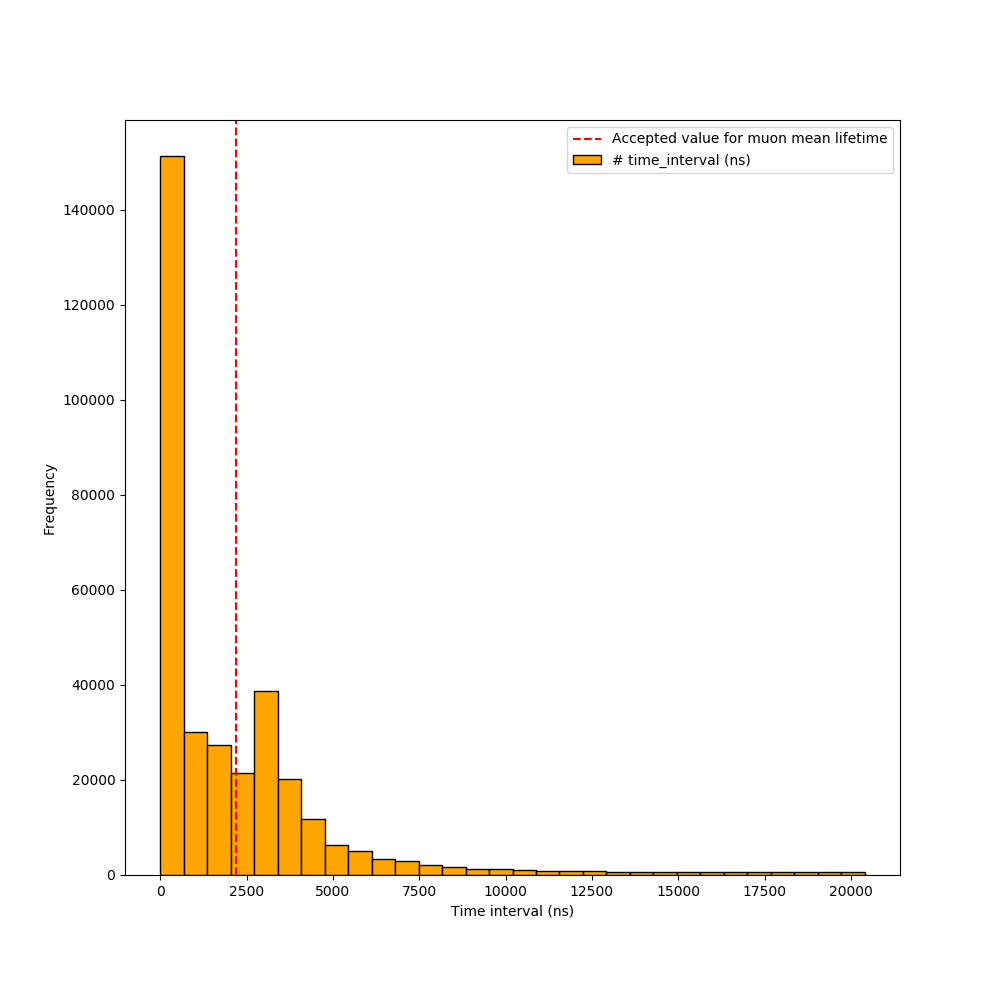
\includegraphics[scale=0.4]{img/data} 
    \caption{Plot of Distribution of Decay Times}
    \label{data}
\end{figure} 
According to \cite{ber}\cite{pat}, the accepted value for the mean lifetime of a muon is $(2.1969811\pm 0.0000022)\times 10^{-6}s$. We have plotted the distribution of the data we collected, along with a vertical line showing this accepted value for the lifetime of a muon in figure \ref{data}.
\begin{figure}[H]
    \centering
    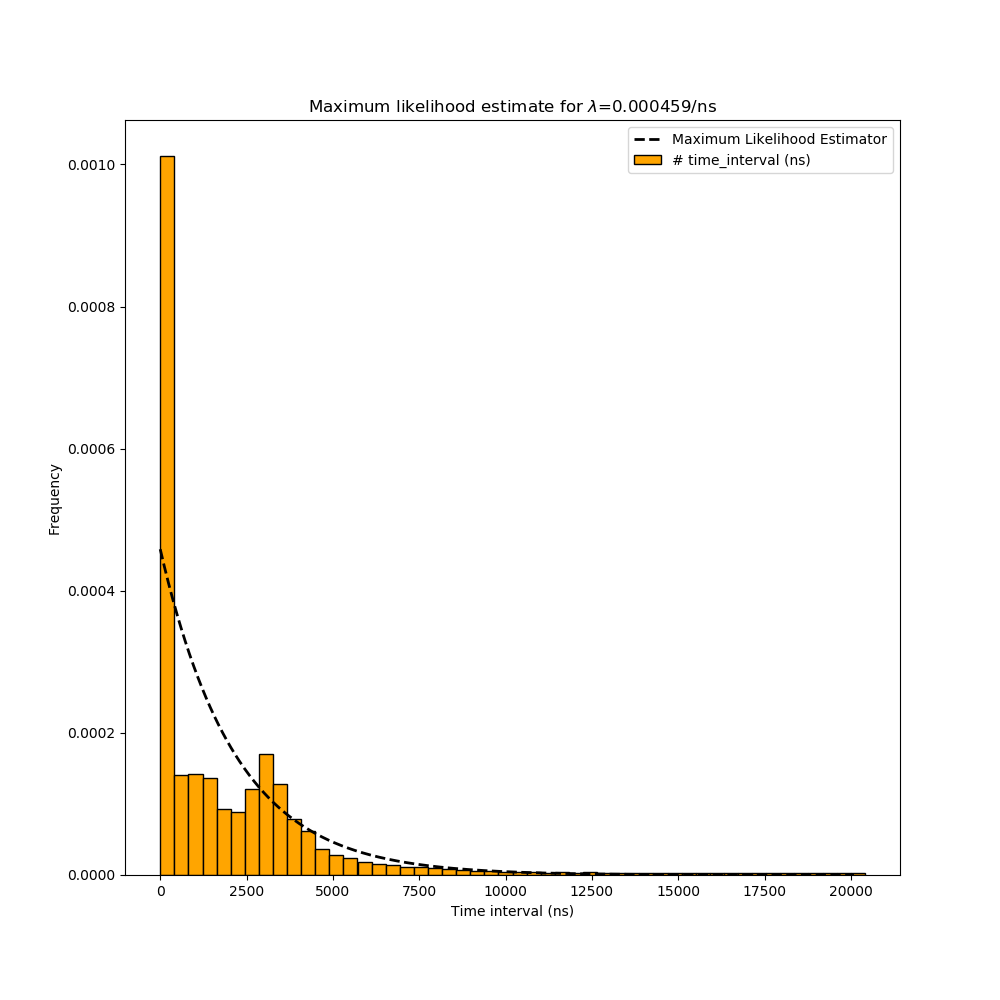
\includegraphics[scale=0.4]{img/mle_estimate} 
    \caption{Plot of Maximum Likelihood Estimate for $\lambda$}
    \label{mle_estimate}
\end{figure} 
In figure \ref{mle_estimate}, we have shown a plot of the data, with the exponential distribution function using the maximum likelihood estimate for the parameter $\lambda$ superimposed. We see a reasonably good fit to the data using this single exponential fit. We also performed this fit using a double exponential, and we were able to get similar results. 

\subsubsection*{Confidence Interval}
Next, we set out to compute the $99$\% confidence interval for our parameter $\lambda$. In order to do this, I need to define a pivot function that is a function of the observations $\{X_i\}$, as well as the parameter $\lambda$. In this case, I used the pivot function:
\begin{align}
        h(X_1,\ldots,X_n, \lambda)=2\lambda \sum_{i=1}^NX_i=\sum_{i=1}^NY_i
\end{align}
where I have defined $Y_i\equiv 2\lambda X_i$. Under this definition for $Y_i$, the distribution of the $Y_i$ is given by the $\chi_2^2$ distribution.\footnote{The proof of this is deferred to appendix A.}

Now, because we assume our $Y_i$ to be i.i.d as the chi-square distribution with 2 degrees of freedom, we have that the distribution function for our pivot function is given by:
\begin{align}
        f_h(x)=f_{\chi^2_{2N}}
\end{align}
Now we need to specify the $\alpha$ we want for our confidence interval. To get the $99$\% confidence interval, we use $\alpha=0.01$. We can now compute the $1-\alpha$ confidence interval for our parameter $\lambda$ using the $\alpha/2$ and $1-\alpha/2$ quantiles of the $\chi_{2n}^2$ distribution. If I define the quantile function for the chi square distribution with $2n$ degrees of freedom to be $\chi_{2n}^2(x)$, then we can compute the confidence interval as:
\begin{align}
        \mathbb{P}\left( \chi_{2n}^2\left(\frac{\alpha}{2}\right)\leq h \leq \chi_{2n}^2\left( 1-\frac{\alpha}{2} \right) \right)=1-\alpha
\end{align}
\begin{align}
        \mathbb{P}\left( \frac{\chi_{2n}^2\left( \frac{\alpha}{2} \right)}{2\sum_{i=1}^nX_i} \leq \lambda \leq \frac{\chi_{2n}^2\left( 1-\frac{\alpha}{2} \right)}{2\sum_{i=1}^nX_i}\right)=1-\alpha
\end{align}
Therefore, we have that our $1-\alpha$ confidence interval is given by:
\begin{align}
        \lambda \in \left[ \frac{\chi_{2n}^2\left( \frac{\alpha}{2} \right)}{2\sum_{i=1}^nX_i}, \frac{\chi_{2n}^2\left( 1-\frac{\alpha}{2} \right)}{2\sum_{i=1}^nX_i}\right]
\end{align}
In the frequentist interpretation, we interpret this by saying the random confidence interval bounds the true [fixed] value of the population parameter $\lambda$ with probability $1-\alpha$. For our case, we had $\alpha=0.01$, $N=335508$, and then we took the sum of our datapoints. When we did this, we got our bounds for the confidence interval to be:
\begin{align}
        \hat{CI} = \left[ 0.000456478, 0.000460556 \right]
\end{align}
As expected, this interval bounds the value for our maximum likelihood estimator.
\begin{figure}[H]
    \centering
    \caption{Plot of 99\% Confidence Interval on Estimate of $\lambda$}
    \label{confidence_intervals}
\end{figure} 
In figure \ref{confidence_intervals}, we plotted the exponential distribution function using the maximum likelihood estimator, as well as the exponential distribution using the upper and lower bounds on the $99$\% confidence interval for $\lambda$. As we can see, the confidence interval is sufficiently tight that one cannot distinguish between the maximum likelihood estimator and the lower and upper confidence interval bounds. 
\begin{figure}[H]
    \centering
    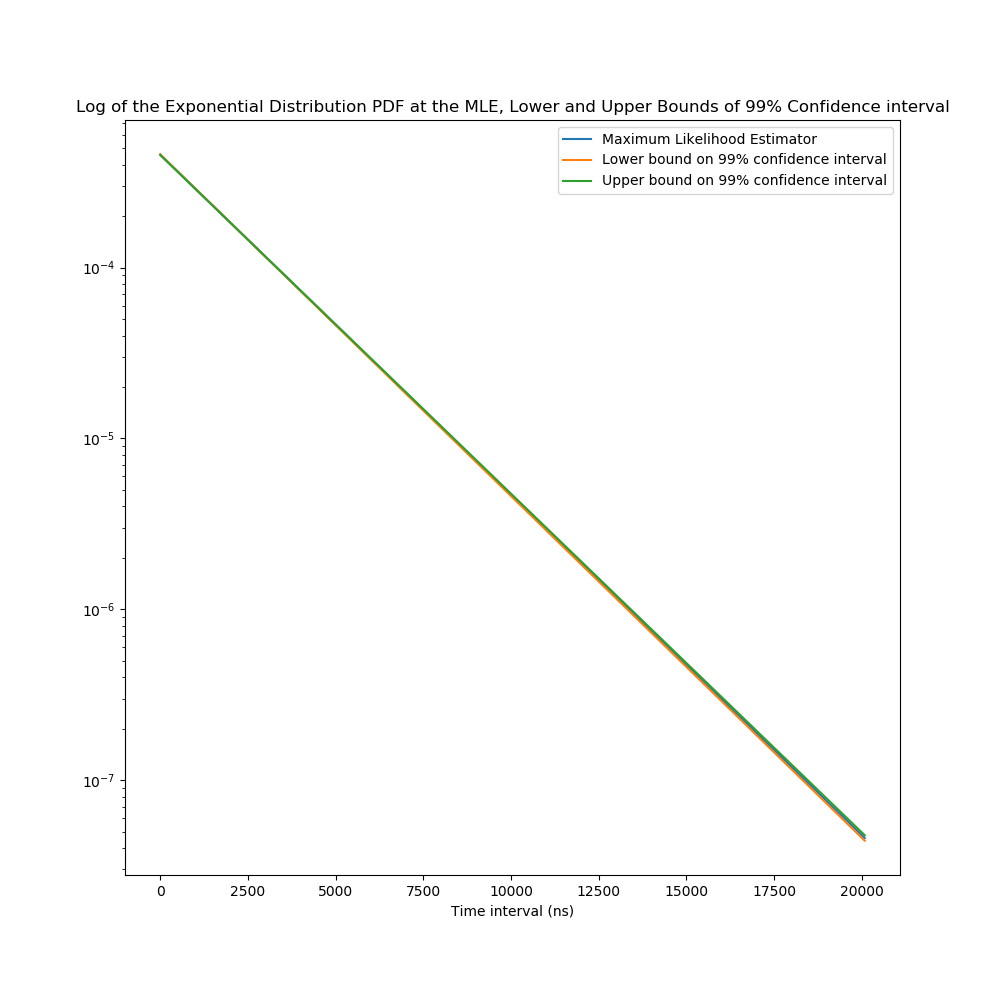
\includegraphics[scale=0.37]{img/log_distributions_confidence_interval} 
    \caption{Plot of Logarithm of 99\% Confidence Interval Distributions}
    \label{log_distributions}
\end{figure} 
In order to see the difference between the distribution functions at the lower and upper bounds on the confidence interval, in figure \ref{log_distributions} we've plotted the logarithm of the distribution functions to try to see some differentiation. At the tail of the distribution, one can make out the difference between the lower and upper bounds.


\subsubsection{Bayesian}
In order to compare different methodologies, we also computed an estimate for the parameter $\lambda$ using a bayesian approach. I used a standard gaussian as the prior, and computed the posterior distribution approximately in order to use the maximum a posteriori estimator as an estimate for the parameter $\lambda$. Note that in the bayesian framework, we do not consider a single ``true'' value of $\lambda$, instead we search for a distribution over all possible values of $\lambda$, and we guess a prior using the so-called nuisance parameters in order to encode our prior beliefs as to the distribution of the values of $\lambda$. We then take a point estimate of the posterior distribution to quote an estimate for the parameter $\lambda$. \\
We use a standard gaussian prior:
\begin{align}
        p(\lambda|\mu,\sigma)=\frac{1}{\sqrt{2\pi \sigma^2}}e^\left( -\frac{(\lambda-\mu)^2}{2\sigma^2} \right)
\end{align}
We use the exponential distribution as our sampling distribution in order to compute the likelihood of the data:
\begin{align}
        L(\mathcal{D}|\lambda)=\prod_{i=1}^N\lambda e^{-x\lambda}
\end{align}
In order to simplify the computations, we used the log posterior distribution instead, in order to get rid of those pesty exponentials:
\begin{align}
        \ell(\lambda|\mathcal{D})=N\log{(\lambda)}-\lambda\sum_{i=1}^Nx_i-\frac{1}{2}\left[ \left( \frac{\lambda-\mu}{\sigma} \right)^2+\log{(2\pi \sigma^2)} \right]
\end{align}

Now, in order to get a point estimate for the parameter $\lambda$, we use the maximum a posterior estimator of our posterior distribution:
The MAP estimator is given by:
\begin{align}
        \hat{\lambda}_{MAP}=\textrm{argmax}_{\lambda}\ell(\lambda \mathcal{D})
\end{align}
So we find the mode of our posterior distribution with respect to $\lambda$:
\begin{align}
        \frac{\partial \ell(\lambda | \mathcal{D})}{\partial \lambda}=\frac{N}{\lambda}-\sum_{i=1}^Nx_i-\left( \frac{\lambda-\mu}{\sigma} \right)\frac{1}{\sigma}=0
\end{align}
Now we solve this for $\lambda$:
\begin{align}
        \lambda^2+\lambda\left( \sum_{i=1}^Nx_i-\frac{\mu}{\sigma^2} \right)-N=0
\end{align}
We can use the quadratic formula \cite{euclid}:
\begin{align}
        \lambda=\frac{\left( \frac{\mu}{\sigma^2}-\sum_{i=1}^Nx_i \right)\pm \sqrt{\left( \sum_{i=1}^Nx_i-\frac{\mu}{\sigma^2} \right)^2-4(1)(-N)}}{2(1)}
\end{align}
\begin{align}
        \lambda=\frac{\frac{\mu}{\sigma^2}-\sum_{i=1}^Nx_i\pm \sqrt{\left( \sum_{i=1}^Nx_i-\frac{\mu}{\sigma^2} \right)^2+4N}}{2}
\end{align}
\begin{figure}[H]
    \flushleft
    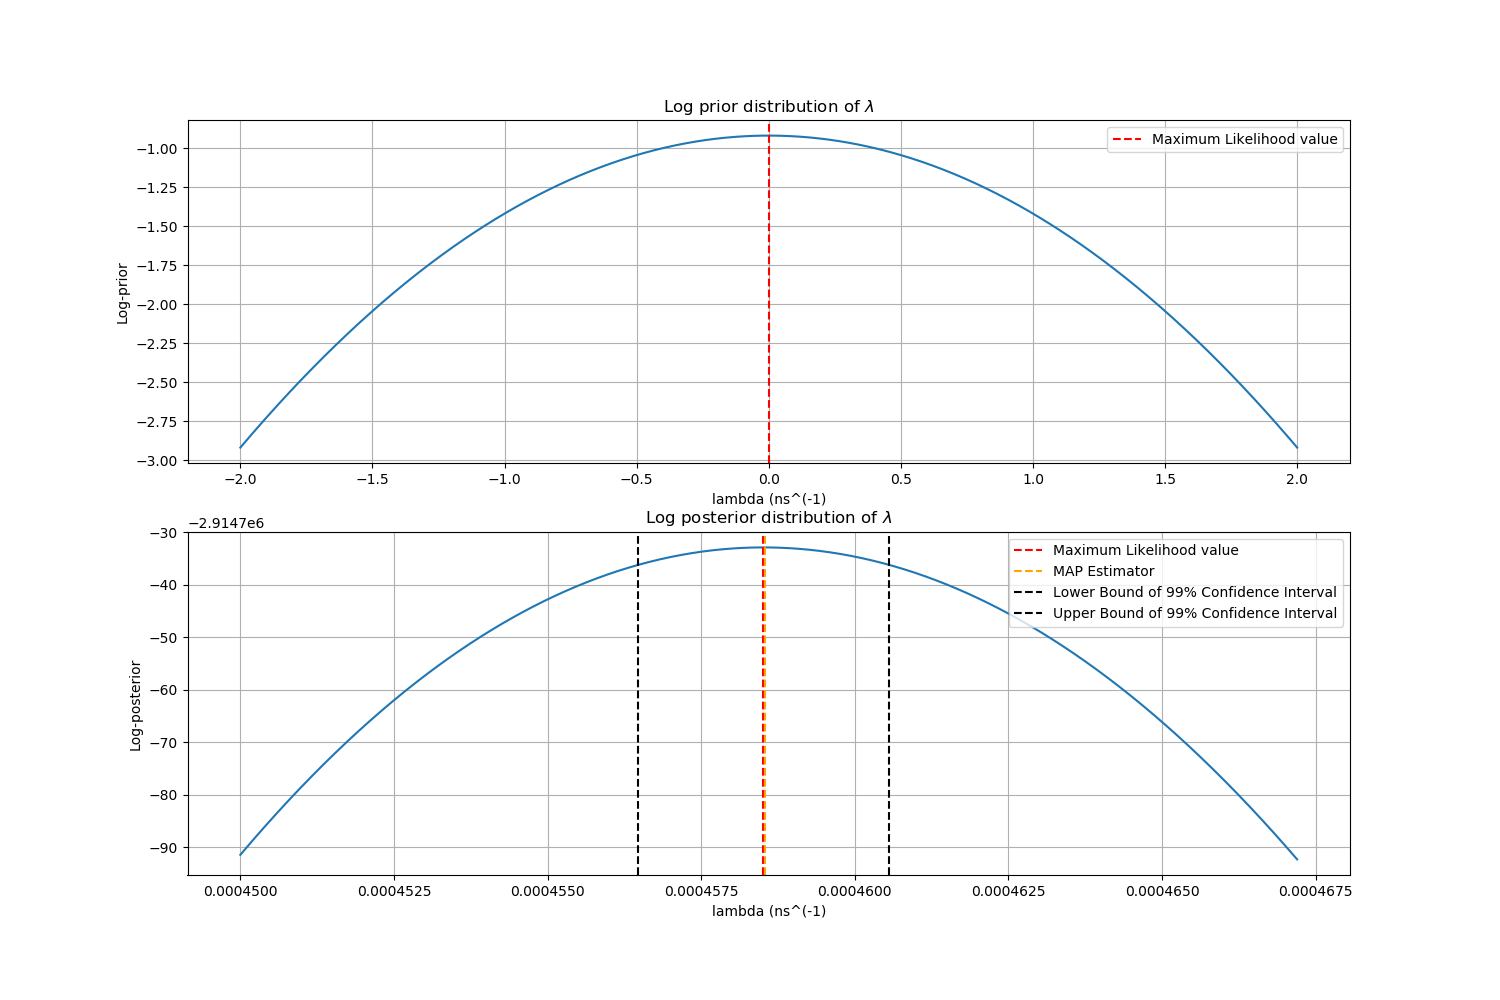
\includegraphics[scale=0.25]{img/prior_versus_posterior} 
    \caption{Plot of Normal Prior on $\lambda$ versus Posterior Distribution}
    \label{prior_versus_posterior}
\end{figure} 

\subsection{Pre-Lab Questions}
\begin{itemize}
        \item[1.] \textit{Question.} Consider an experiment that counts the number of events in a given amount of time. Suppose that, after many repetitions of the experiment, you find that the average number of events in a given amount of time is $\nu$. What is the standard deviation of the results in your experiment?
        
        \textit{Answer.} Consider the sequence of random variables: $\{X_1,\ldots,X_n\}$. This random process represents our experiment. If we assume the $X_i$ are i.i.d and Poisson distributed, then we know we are looking for an estimate for the parameter $\lambda$. In this case, we are told that empirical mean of the data is $\nu$. For a Poisson distributed random variable, the variance is $\lambda$, so the standard deviation is $\sqrt{\lambda}$. 
        \item[2.] \textit{Question.} Suppose the count rate (events/sec) from the two detectors in the muon experiment are $R_1$ and $R_2$. What is the rate of accidental coincidences if the width of the coincidence window (measured in seconds) is W?
        
        \textit{Answer.} We understand that accidental coincidences are excluded by the XOR gate. Therefore the rate of accidental coincidences is simply the probability of events which satisfy the XOR condition. The XOR condition in this lab is the occurrence of muons triggering detectors A and B but not A AND B. Therefore the probability of accidental coincidences is
        \begin{align}
            P_{Acc.} = P(A\cap B).
        \end{align}
        Given a coincidence window of $W$ and that the two detectors A and B have count rates $R_1$ and $R_2$ respectively. We know that the number of counts in A and B are
        \begin{align}
            |A| &= R_1 W \\
            |B| &= R_2 W.
        \end{align}
        Therefore the probability $P(A\cap B$ is a function of $R_1, R_2,$ and $W$. Therefore
        \begin{align}
            P_{Acc.} = P(A\cap B) = P(A(R_1, W))P(B(R_2, W)).
        \end{align}
        Using the previously justified Poisson distribution, we can expand this probability as follows.
        \begin{align}
            \begin{split}
                P_{Acc.} &= P(N=|A|=R_1W | \lambda = \nu) \\
                &\times P(N=|B|=R_2W, \lambda = \nu) 
            \end{split} \\
            &= \frac{\nu^{R_1 W}e^{-\nu}}{(R_1 W)!}\frac{\nu^{R_1 W}e^{-\nu}}{(R_2 W)!} \\
            &= \frac{\nu^{W(R_1 + R_2)}e^{-2\nu}}{(R_1W)!(R_2W)!}.
        \end{align}
        Given count rates of $R_1$ and $R_2$, this is the probability (or rate) of accidental coincidences if the width of the coincidence window is $W$.
        
        \item[3.] \textit{Question.} How can the result of question 2 allow you to improve your count rate without significantly increasing the noise in your experiment?
        
        \textit{Answer.} To maximize the signal to noise ratio of the experiment, we need to minimize equation (10) as a function of $W$. A procedure for doing this is to try different values of $W$ until $P_{Acc.}$ is minimized. 

        \item[4.] \textit{Question.} Assume events occur at a particular rate $R$ (events/s). If you start looking for events at some time ($t=0$), what is the probability that the first event you detect occurs between times $T$ and $T+\Delta T$? Assume that $\Delta t$ is a small interval of time so that $R\Delta T<<1$. Hint: First calculate the probability that zero events occur in the time interval $T$.
        
        \textit{Answer.} This is a Poisson process since $R\Delta T << 1$. Therefore the probability that the first event occurs within the range $T$ and $T + \Delta T$ is
        \begin{align}
            P_{(T + \Delta T)} = R\Delta T \times e^{-R\Delta T}.
        \end{align}
        
\end{itemize}

%The analysis or your data should always include an error analysis,
%providing an estimate of the experimental uncertainty in any measured
%quantities.  If computer programs are used for analysis, they should be
%included in an appendix. 

%In the analysis, indicate the formulas used, the units of each
%quantity entering the equations, and a numerical example for each
%computation. You should clearly distinguish statistical and 
%systematic error  and indicate how the assignment of error
%was made.  Graphs should be presented with the error of each
%experimental point indicated (either in the graph or in the caption or text).
